\documentclass{beamer}

%----------------------------------------------------------------------------
% Präambel
%----------------------------------------------------------------------------

\usetheme[progressbar=frametitle]{metropolis}

\usepackage[ngerman]{babel} % deutsches Sprachpaket wird geladen
\usepackage[T1]{fontenc} % westeuropäische Codierung wird verlangt
\usepackage{hyperref} % Um diverse Verlinkungen zu erzeugen 
\usepackage{appendixnumberbeamer} % Damit das \appendix einen eigenen Zähler hat

%\setbeamertemplate{caption}[numbered] % set captions with numbers

\usepackage{amssymb}

\newcommand{\new}[1]{{\color{red}#1}}
\title[UPerNet]{UPerNet}
\subtitle{Unified Perceptual Parsing Network}
\author[Göbl, Schäfer, Scheib]{Lukas Göbl, Peer Schäfer, Lukas Scheib}
\institute{Computer Vision Journal Club\\
University of Cologne}
\date{03.07.2025}

\setbeamertemplate{footline}{}%[page number]
\setbeamercolor{framesource}{fg=gray}
\setbeamercolor{footnote}{fg=gray}
\setbeamerfont{framesource}{size=\tiny}
\setbeamerfont{footnote}{size=\tiny}
\renewcommand{\footnoterule}{}

%Standard footer definition:
\setbeamertemplate{navigation symbols}{
    \parbox{\linewidth}{
    \vskip1pt
    \textcolor{gray}{%
        \tiny
        \hfill \insertshortauthor~\vline~\insertshorttitle~\vline~\insertframenumber/\inserttotalframenumber\quad
        }
    \vskip3pt
    }
}

%New command for footnotes without counter
\newcommand\blfootnote[1]{
  \begingroup
  \renewcommand\thefootnote{}\footnote{#1}
  \addtocounter{footnote}{-1}
  \endgroup
}

\begin{document}

%\iffalse
\begingroup
\setbeamertemplate{navigation symbols}{}
\maketitle
\endgroup
\addtocounter{framenumber}{1}
%\fi

\begin{frame}{Experiment 1: Standard Semantic Segmentation}
  Comparison with state-of-the-art methods for semantic segmentation of objects on the ADE20K dataset:
  \begin{figure}
    \centering
    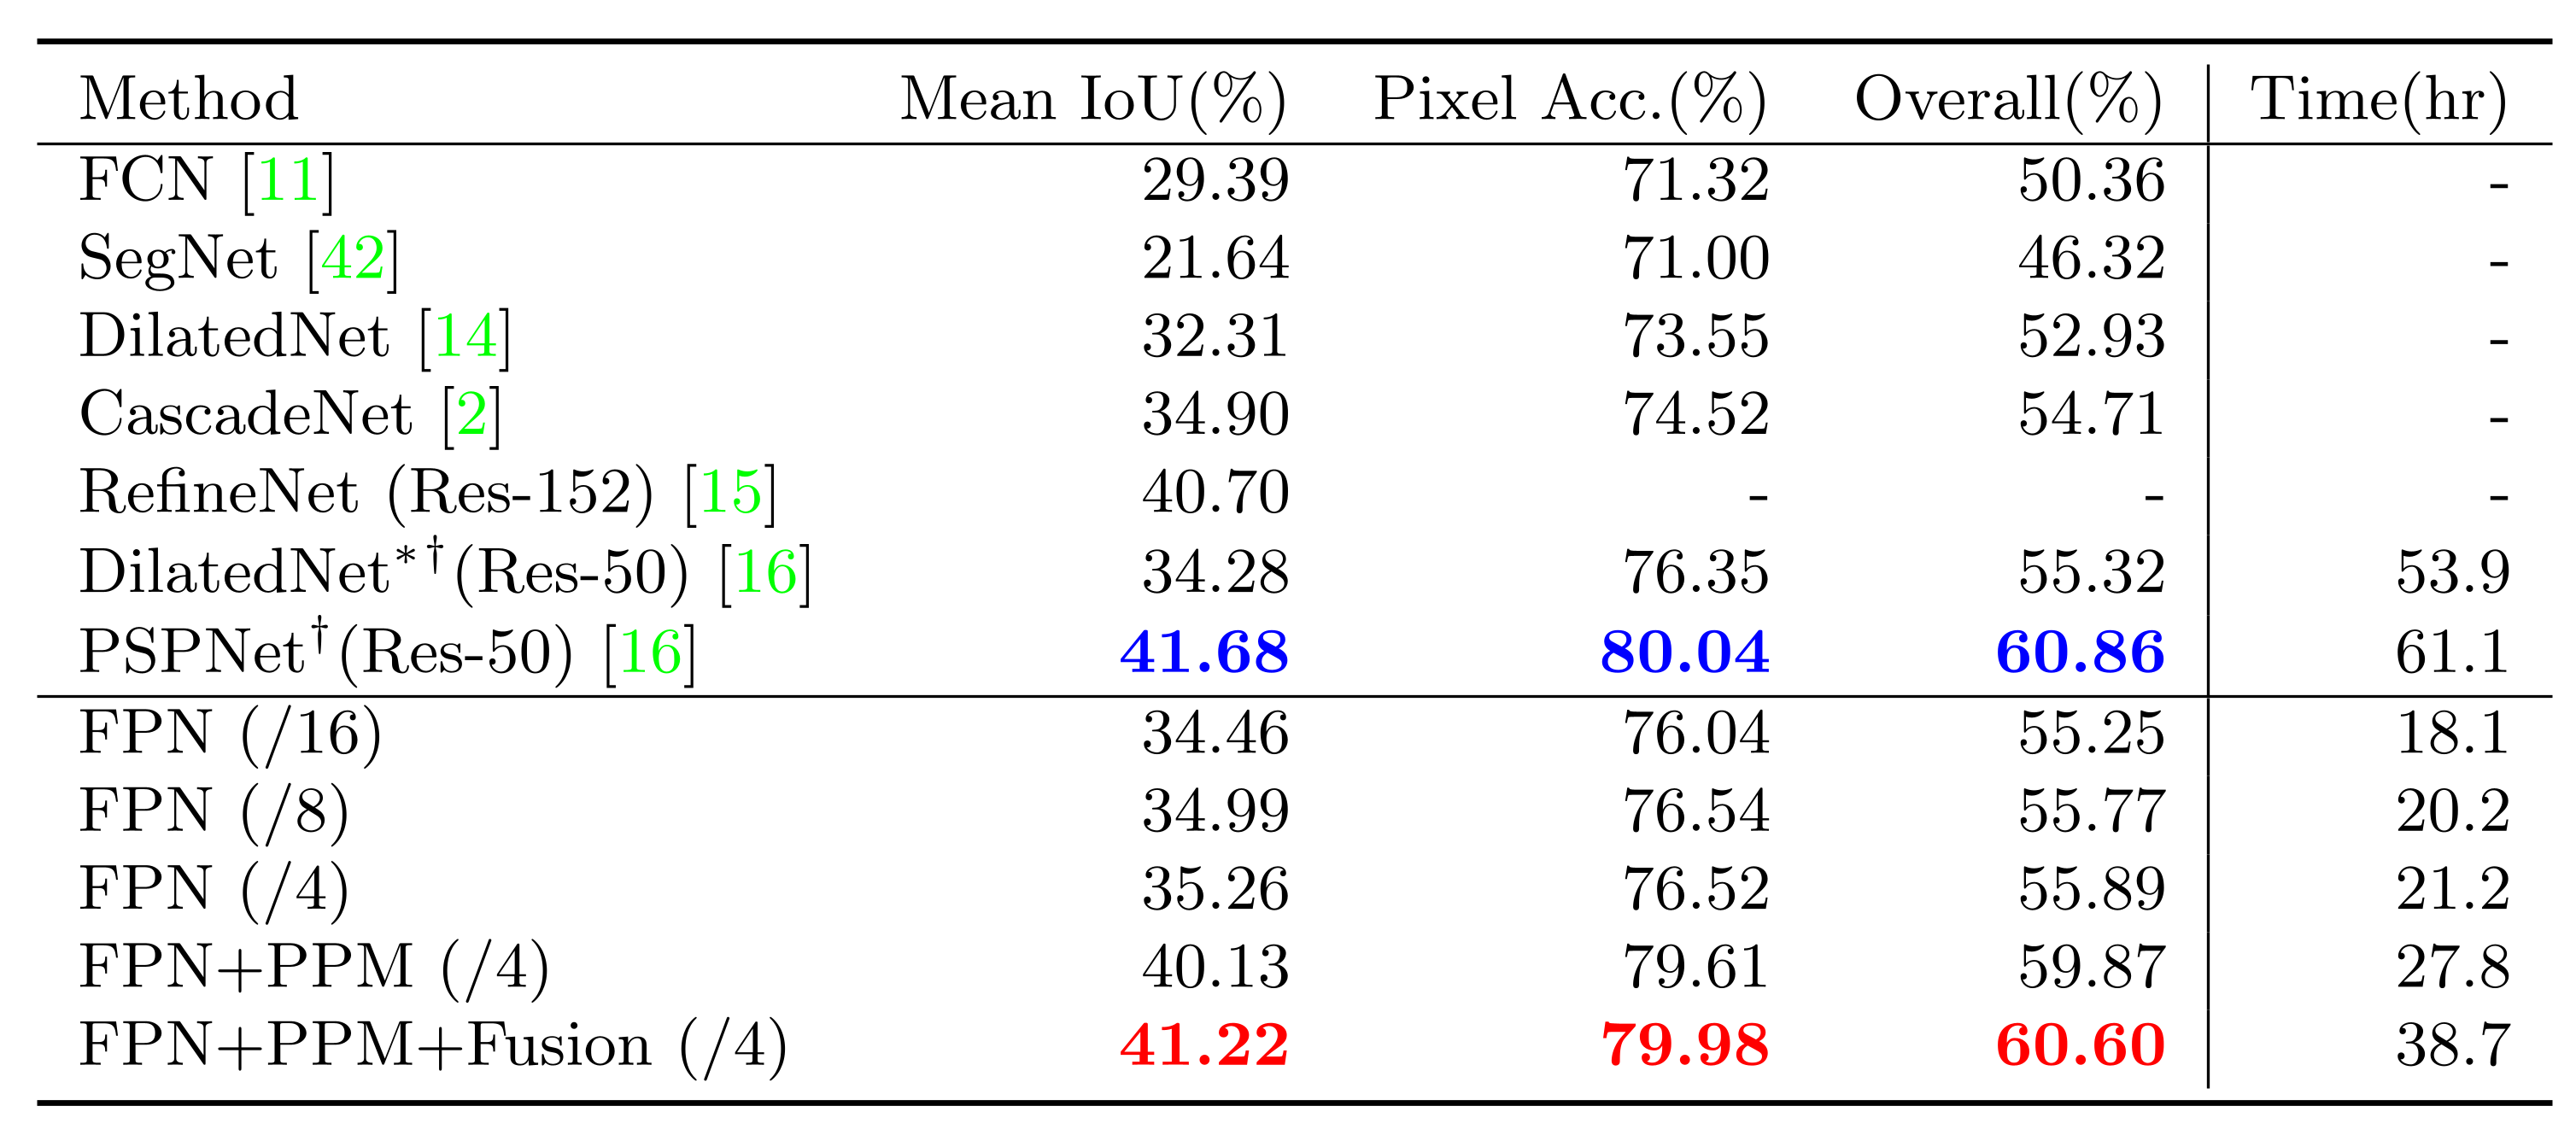
\includegraphics[width=\textwidth]{Images/Table2.png}
    \blfootnote{\href{https://doi.org/10.48550/arXiv.1807.10221}{Xiao et al. (2018), Table 2}}
  \end{figure}
\end{frame}

\begin{frame}{\new{Notizen}}
  \footnotesize
  \begin{itemize}
    \item Warum bezeichnen die DilatedNet als "\emph{strong baseline reference}"?
    \item Evtl. Metriken erklären
    \item "\emph{Further increasing resolution of feature maps brings consistent gain. PPM is highly compatible with FPN. Empirically we find that fusing features from all levels of FPN yields best performance.}"
    \item "\emph{The performance of FPN is surprising considering its simplicity with feature maps being simply up-sampled by bilinear interpolation instead of time-consuming deconvolution, and the top-down path is fused with bottom-up path by an 1x1 convolutional layer followed by element-wise summation without any complex refinement module.}"
    \item Was ist der Unterschied zwischen dem Task, den die machen ("\emph{semantic segmentation, we report the results trained on ADE20K using object annotations}") und object classification?
    \item Was heißt "\emph{Our results are obtained without multi-scale inference or other techniques.}"?
  \end{itemize}
\end{frame}

\begin{frame}{Experiment 2: Unified Perceptual Parsing}
  Results of UPP on the Broden+ dataset:
  \begin{figure}
    \centering
    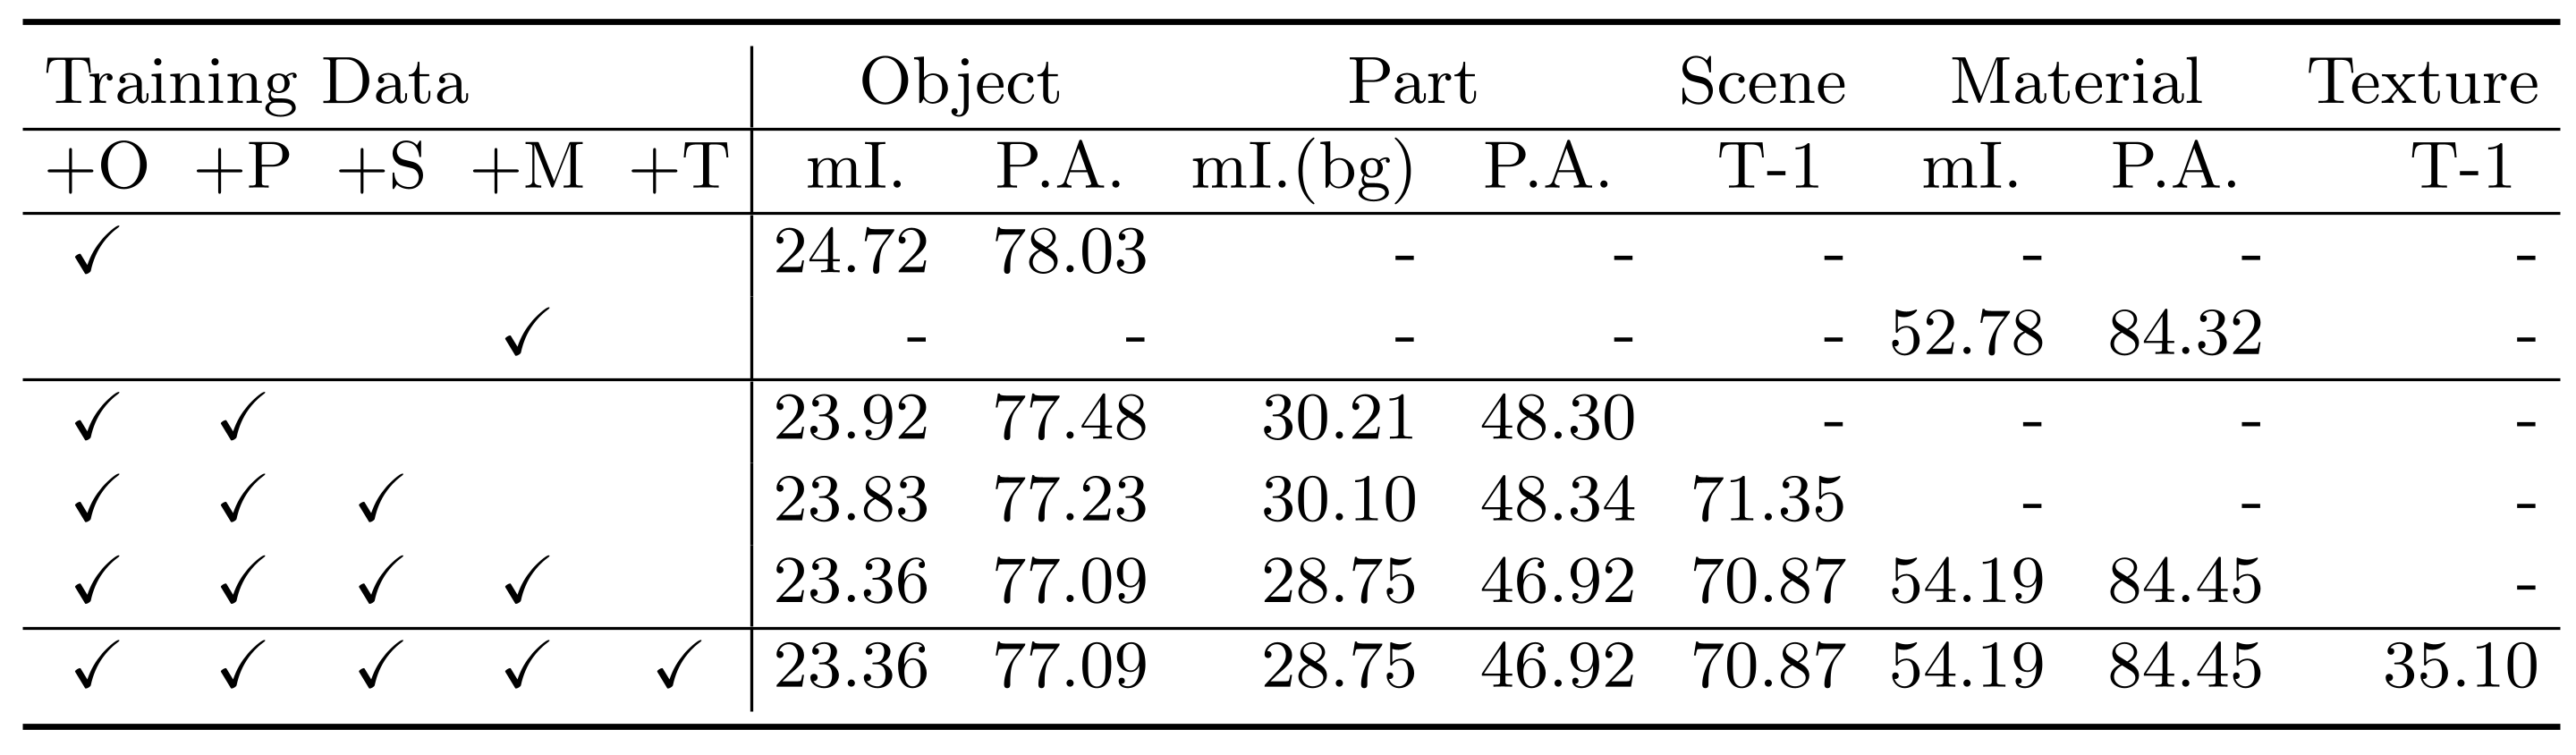
\includegraphics[width=\textwidth]{Images/Table3.png}
    \blfootnote{\href{https://doi.org/10.48550/arXiv.1807.10221}{Xiao et al. (2018), Table 3}}
  \end{figure}
  \vspace{-1cm}
  \begin{itemize}
    \item Joint training across 5 perceptual levels
    \item Performance remains stable for most tasks and even improves for material
    \item Texture prediction requires fine-tuning due to different data distribution
  \end{itemize}
\end{frame}

\begin{frame}{Experiment 2: Unified Perceptual Parsing}
  Some qualitative results:
  \vspace{-0.25cm}
  \begin{figure}
    \centering
    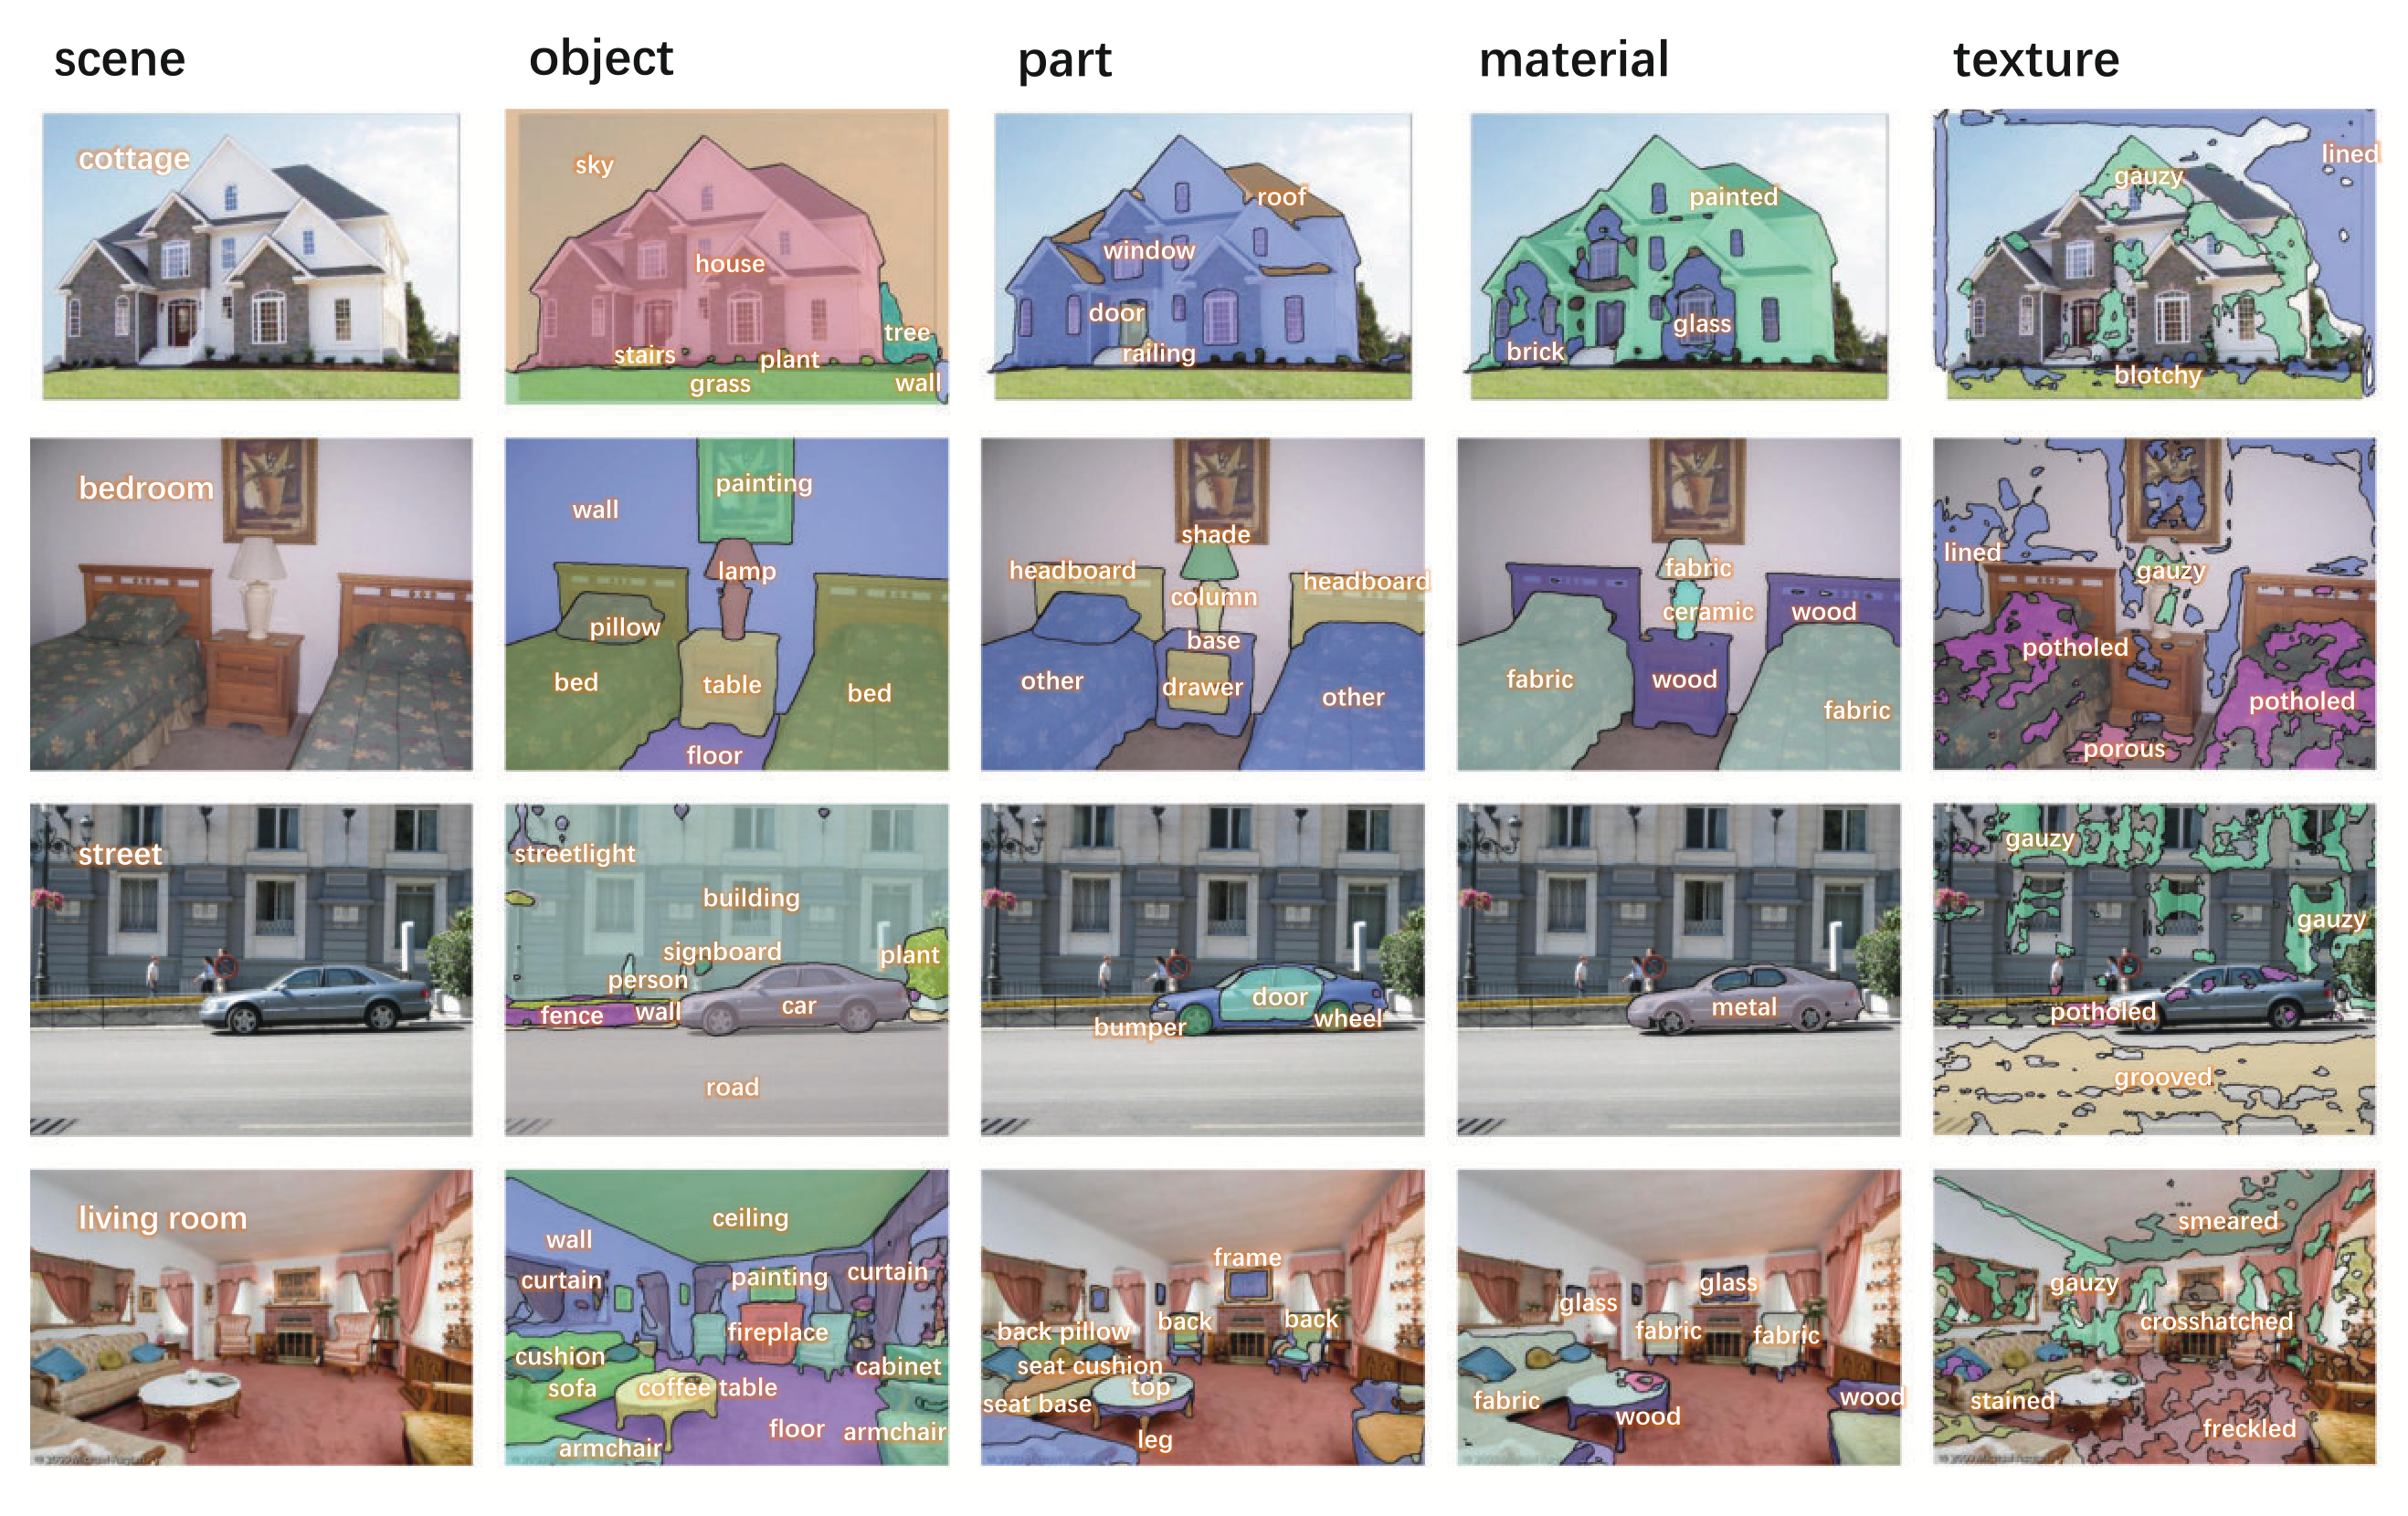
\includegraphics[width=\textwidth]{Images/Figure5 Springer.png}
    \blfootnote{\href{https://doi.org/10.1007/978-3-030-01228-1_26}{Xiao et al. (2018), Figure 5}}
  \end{figure}
  \vspace{-1cm}
\end{frame}

\begin{frame}{Model Inspection: Discovering Visual Knowledge}
  Visualization of scene-object relations after clustering:
  \vspace{-0.25cm}
  \begin{figure}
    \centering
    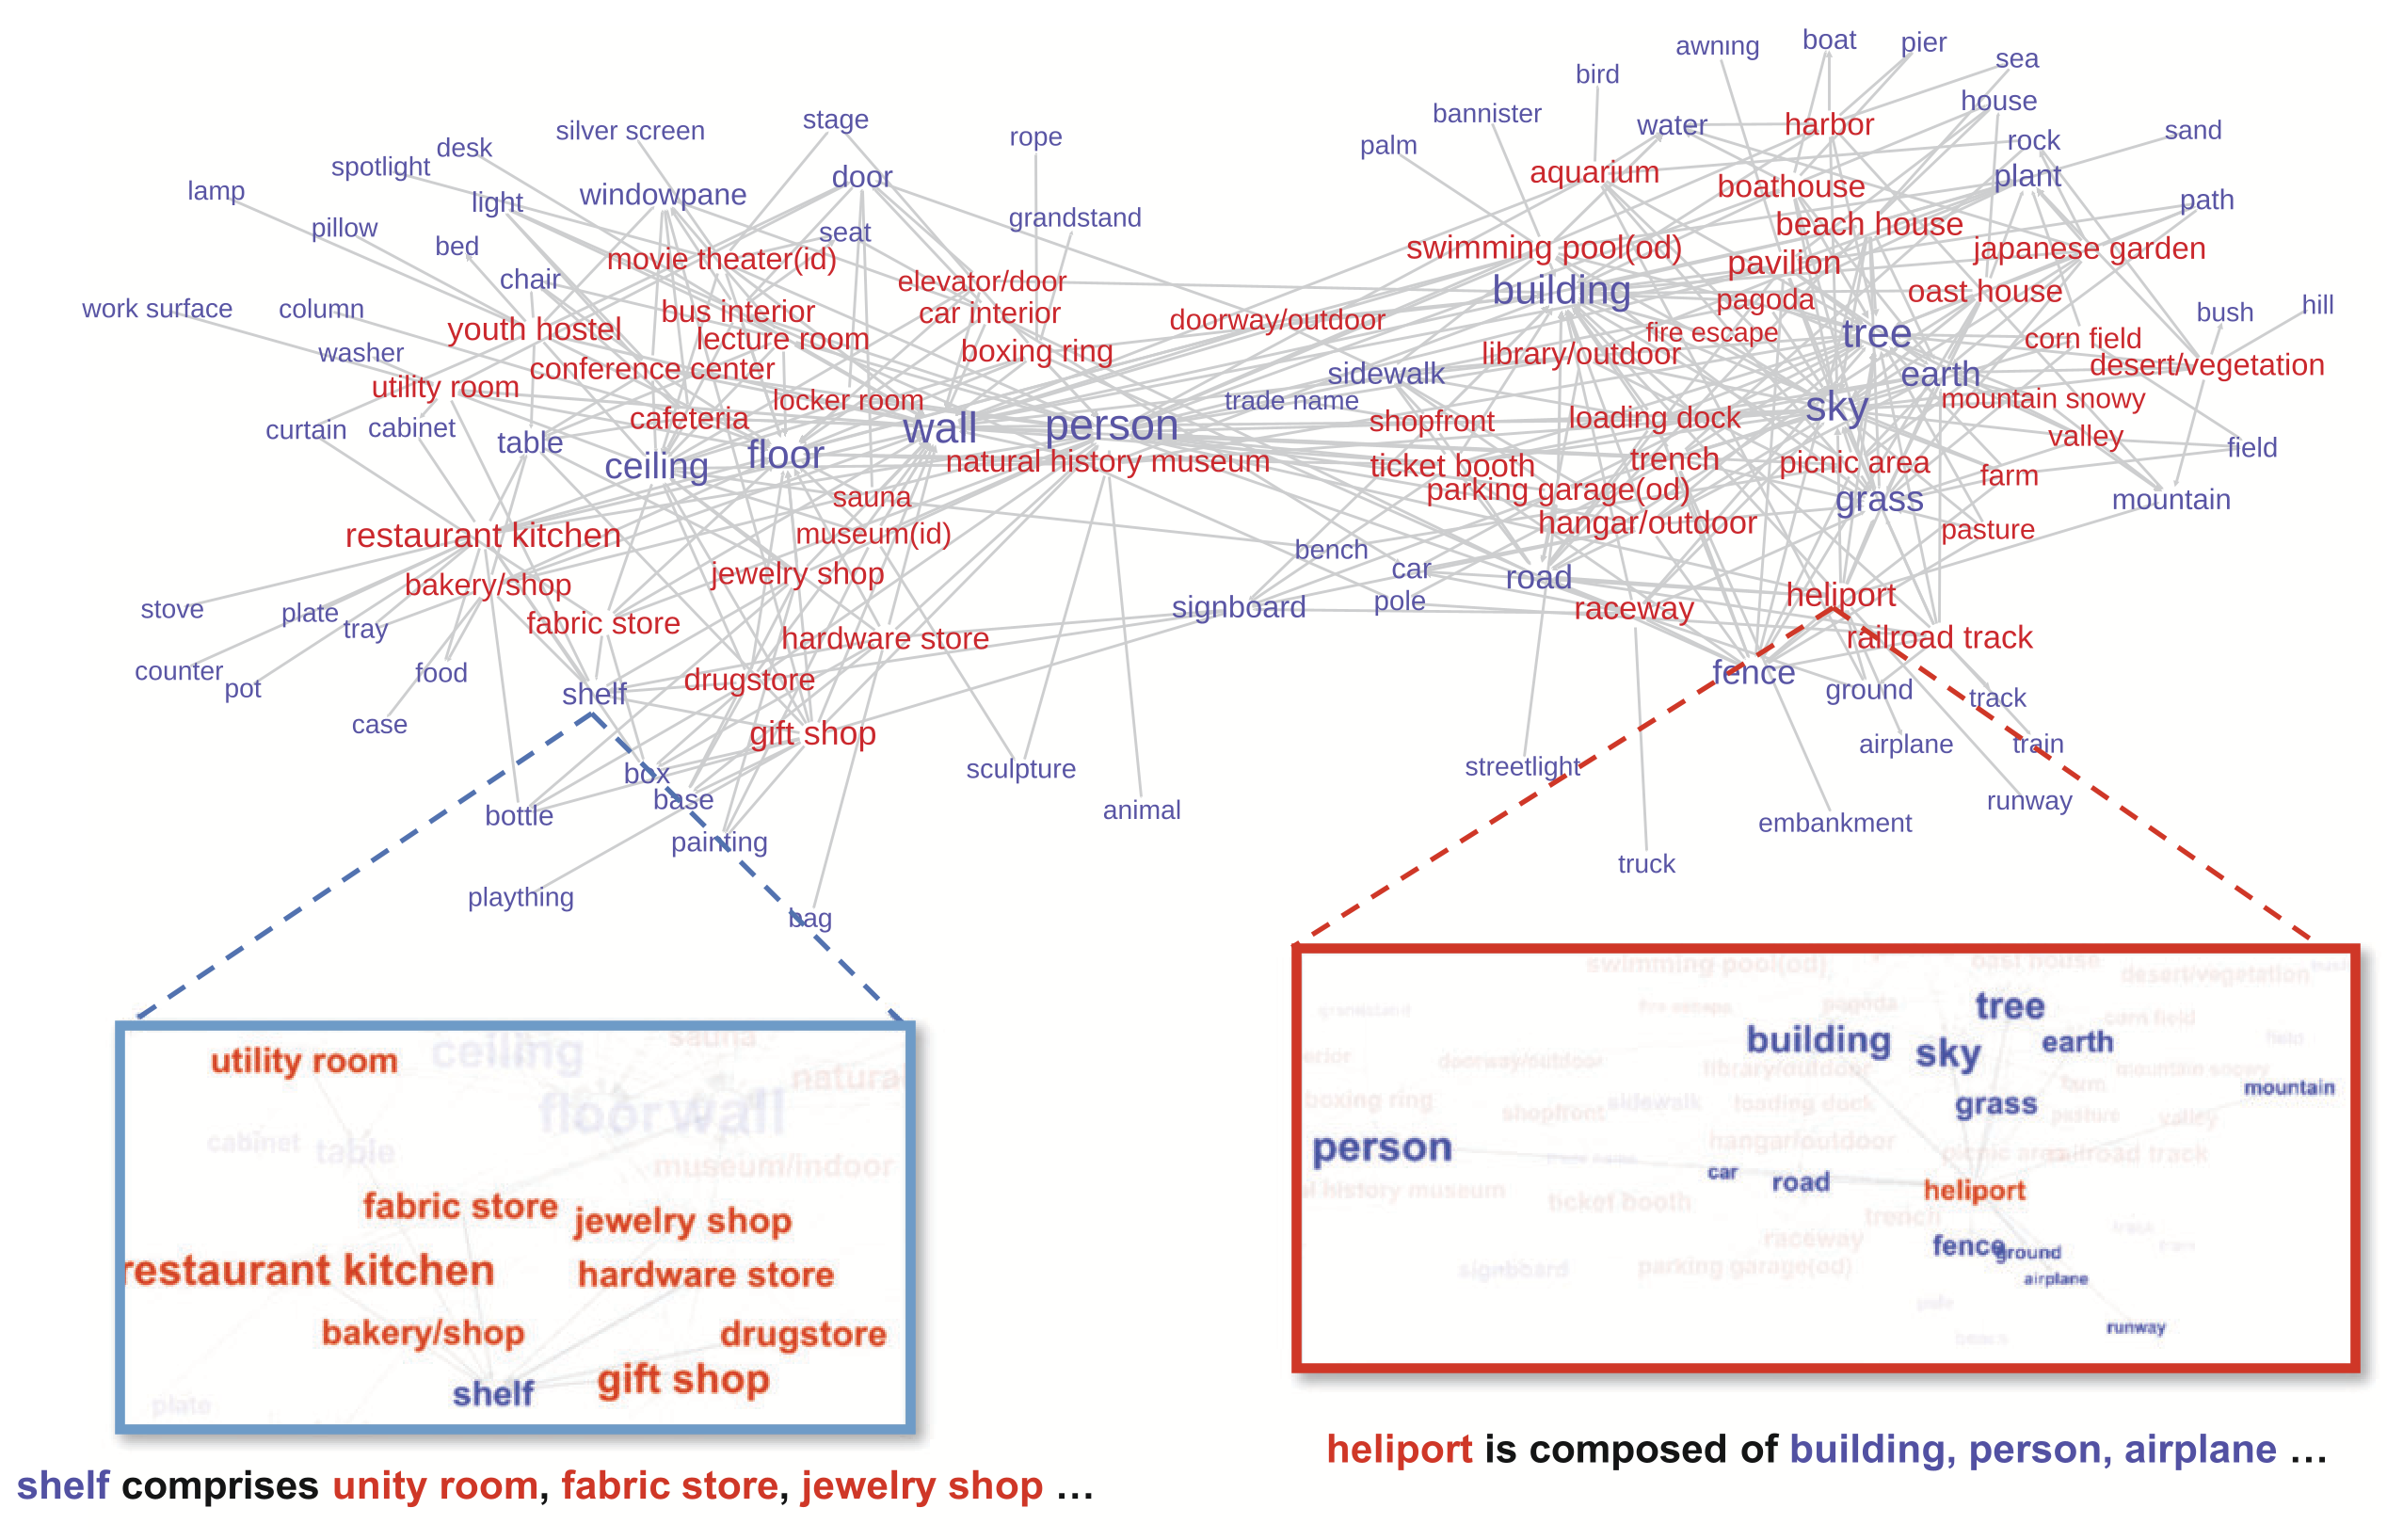
\includegraphics[width=\textwidth]{Images/Figure6a.png}
    \blfootnote{\href{https://doi.org/10.48550/arXiv.1807.10221}{Xiao et al. (2018), Figure 6a}}
  \end{figure}
  \vspace{-1cm}
\end{frame}

\begin{frame}{Model Inspection: Discovering Visual Knowledge}
  \begin{figure}
    \centering
    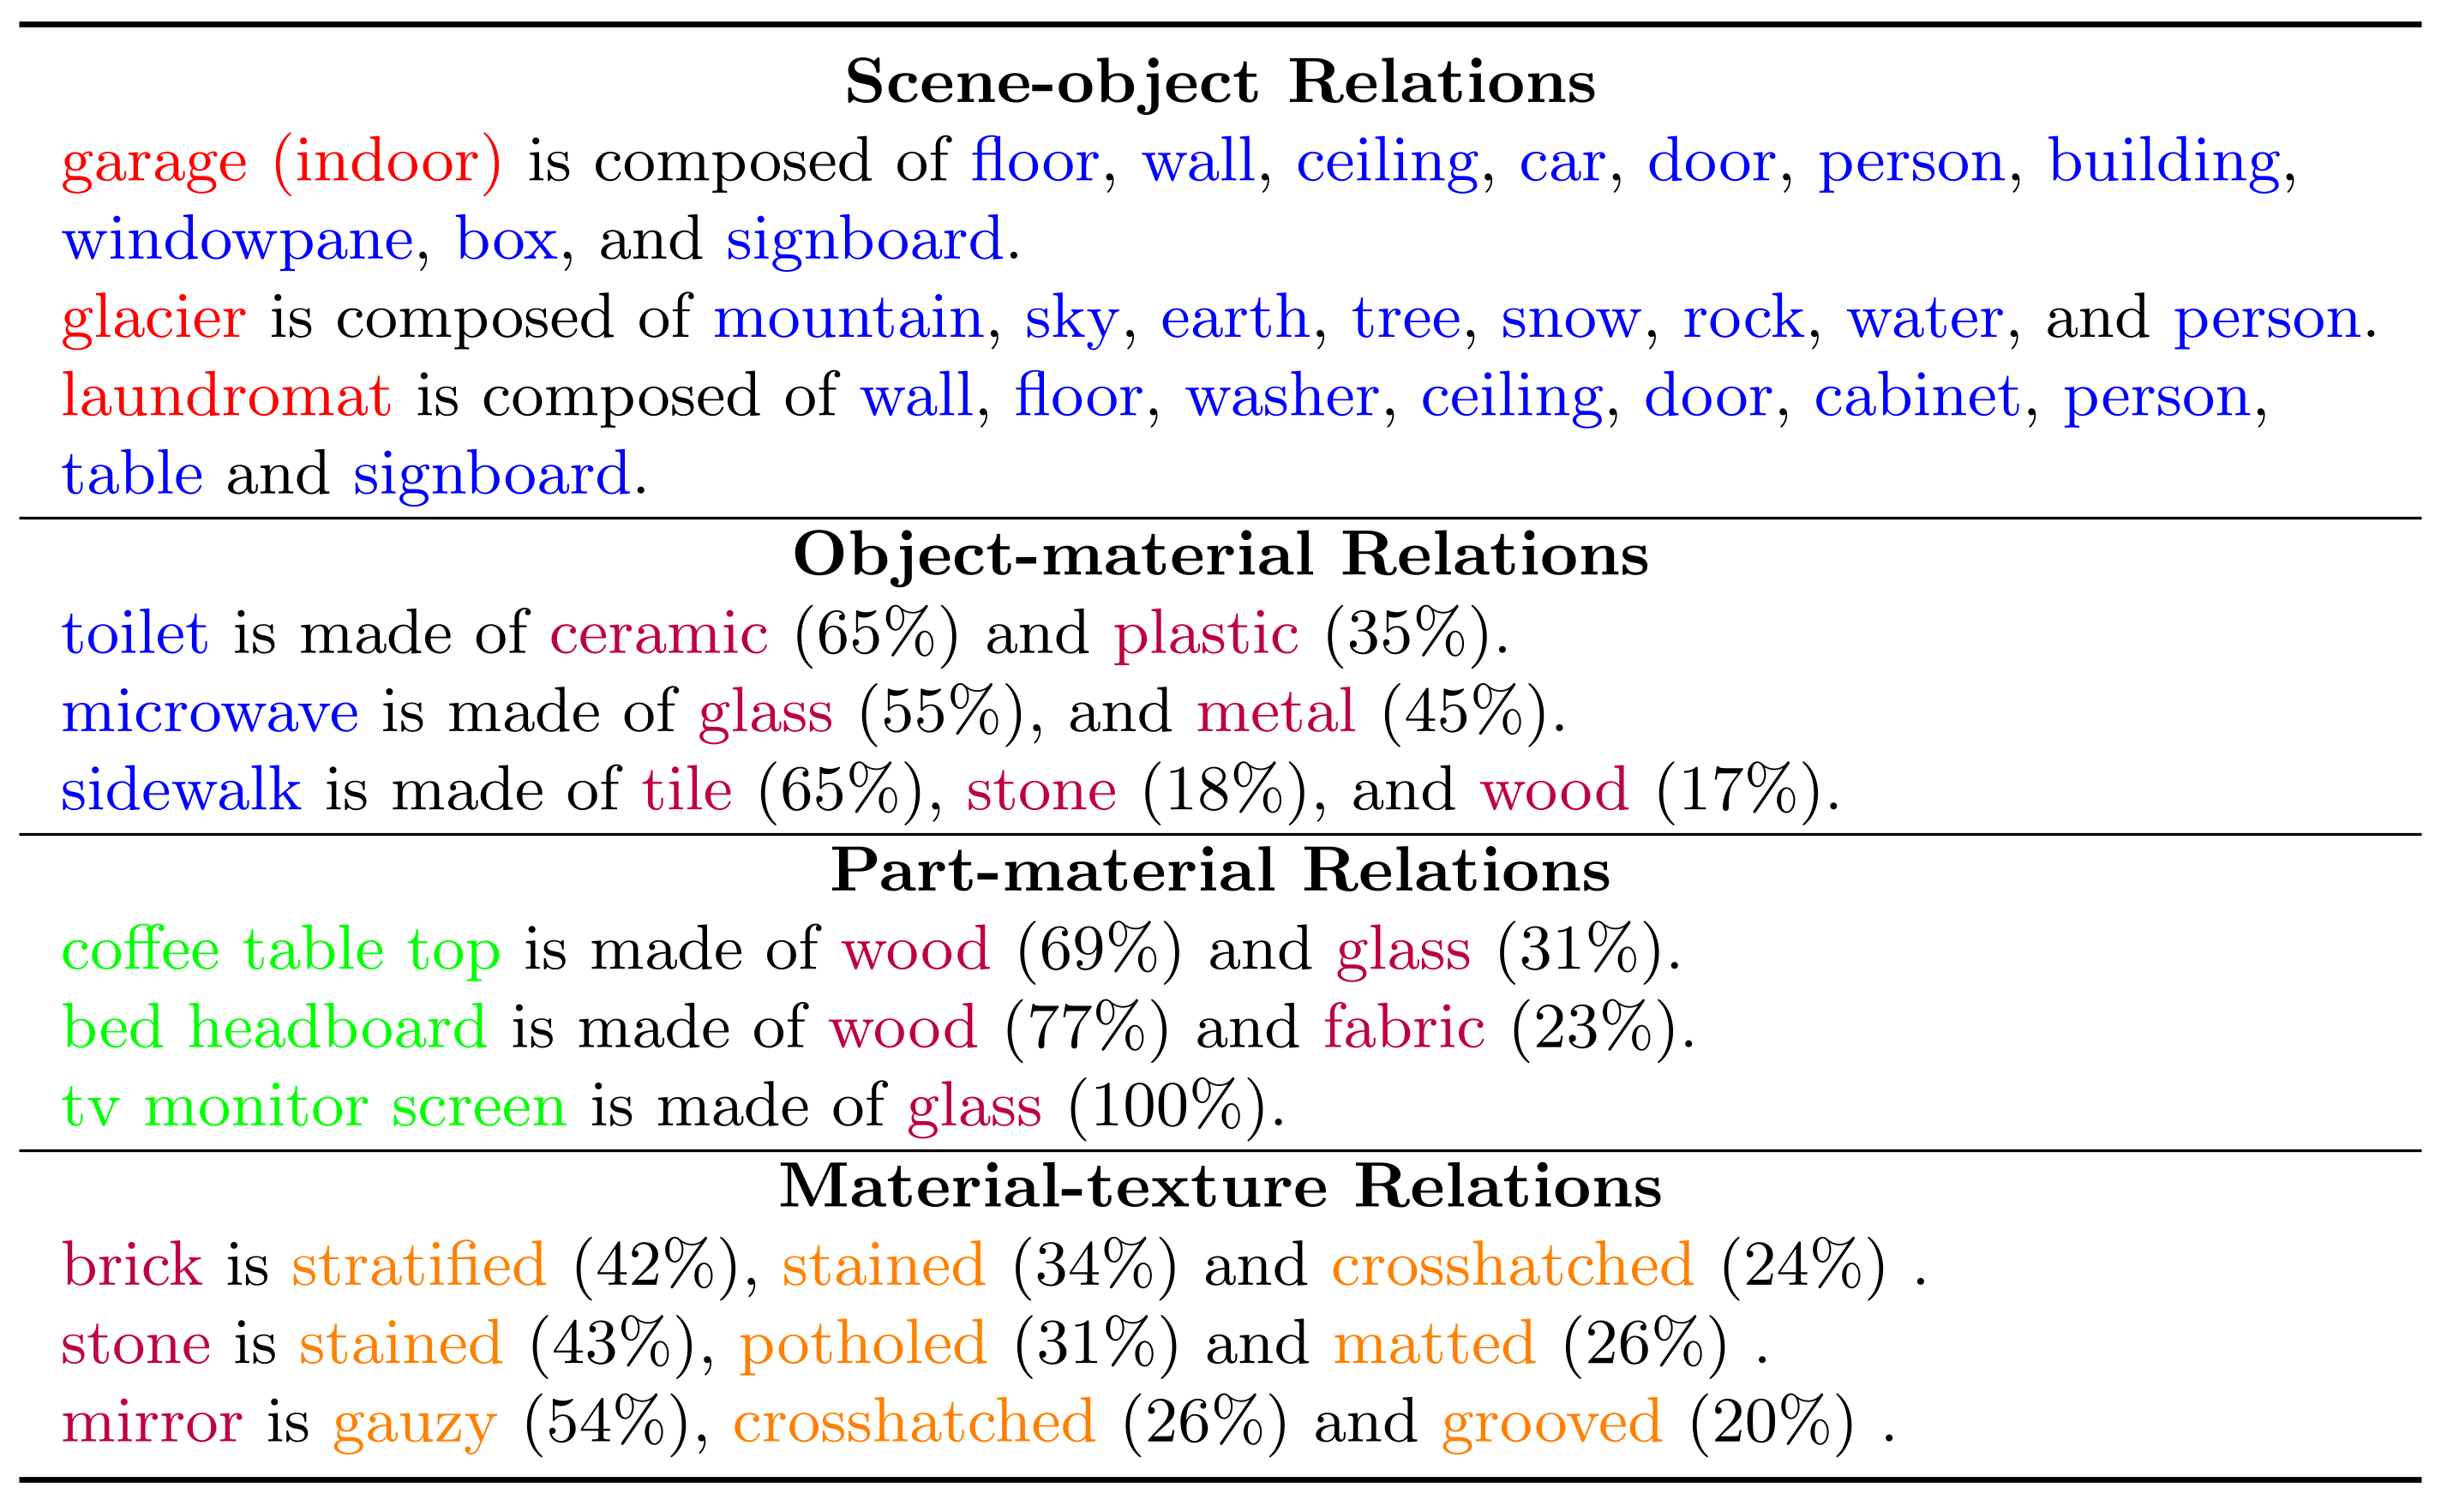
\includegraphics[width=\textwidth]{Images/Table4.png}
    \blfootnote{\href{https://doi.org/10.48550/arXiv.1807.10221}{Xiao et al. (2018), Table 4}}
  \end{figure}
\end{frame}

% Slide 4 – Conclusion and Perspective
\begin{frame}{Conclusion and Perspectives}
  \begin{itemize}
    \item UPerNet performs competitively on semantic segmentation with less training time
    \item The network can handle heterogeneous annotations and tasks across multiple perception levels
    \item Allows for discovery of compositional visual knowledge (e.g. scene-object-material relations)
    \item Future directions:
    \begin{itemize}
      \item Better integration of image-level and pixel-level annotations
      \item Applications in explainable AI and reasoning
    \end{itemize}
  \end{itemize}
\end{frame}

% Slide 5 – Open Questions
\begin{frame}{\new{Open Questions}}
  \begin{itemize}
    \item How does the model handle conflicting or incomplete labels in heterogeneous data?
    \item What are the limitations in terms of generalization to unseen scenes or rare materials?
    \item \new{...}
  \end{itemize}
\end{frame}


\end{document}